\documentclass[letterpaper, 11pt]{article}

\usepackage{amsmath, amsthm, latexsym, amssymb, graphicx, bold-extra, mathrsfs, frcursive}
\usepackage[pdftex]{color}
\usepackage[T1]{fontenc}
\usepackage{listings}
\usepackage{adjustbox}
\usepackage{hyperref}
% Simplifies margin settings
\usepackage{geometry}
\geometry{margin=1in}

% Puts list item indicators in bold; makes flush with previous margin
\renewcommand\labelenumi{\bf\theenumi.}
\renewcommand\labelenumii{\bf\theenumii.}
% setlength\leftmargini{1.4em}
\setlength\leftmarginii{1.4em}

% Flexibility for headers and footers
\usepackage{fancyhdr}
\pagestyle{fancyplain}
\fancyhf{} %clear all header and footer fields
\lhead{\bf \small How To Write Fast Numerical Code \hspace*{\fill} Page \thepage}
\headsep 0.2in
\thispagestyle{empty}
\renewcommand{\headrulewidth}{0pt}
\renewcommand{\footrulewidth}{0pt}

\parindent 0in
\parskip 10pt
\setlength{\headheight}{20pt}

\title{ETH Zurich}

\begin{document}

%=======================================

\begin{center}
\Large \bf 263-2300-00: How To Write Fast Numerical Code

\Large \bf Assignment 3: 100 points

\large Submitted by Jinank Jain
\end{center}

\textbf{Solution 1}\\ \\
\textbf{Some technical details about test setup:}
\begin{itemize}
\item Compiler: clang-800.0.42.1
\item Machine: MacOSX Intel(R) Core(TM) i7-3520M CPU @ 2.90GHz
\item Processor Generation: Ivy Bridge
\item Flags: -O3 -fno-tree-vectorize -mavx -mavx2 -msse4.1
\end{itemize}
\begin{figure}[h!]
    \centering
    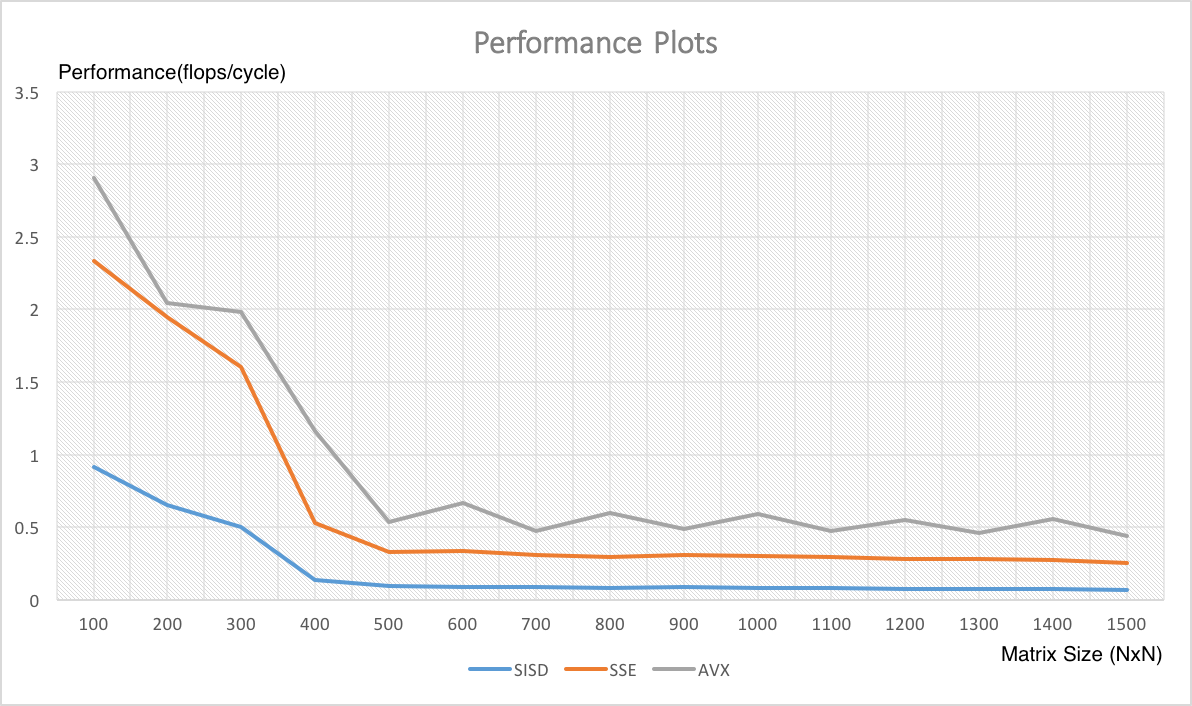
\includegraphics[width=100mm]{ques1}
    \caption{Plots for comparing SISD, SSE, and AVX implementation.}
    \label{fig:runtime}
\end{figure}
\begin{table}[]
\centering
\label{table1}
\begin{tabular}{|c|c|c|c|c|c|}
\hline
N    & SISD      & SSE      & AVX      & Speed Up (SSE/SISD) & Speed Up (AVX/SSE) \\ \hline
100  & 0.91 & 2.33 & 2.90 & 2.55         & 1.24        \\ \hline
200  & 0.65 & 1.94 & 2.04 & 2.97         & 1.05        \\ \hline
300  & 0.50 & 1.60 & 1.97 & 3.19         & 1.23        \\ \hline
400  & 0.13 & 0.52 & 1.16 & 3.84         & 2.20        \\ \hline
500  & 0.09 & 0.33 & 0.53 & 3.58         & 1.62        \\ \hline
600  & 0.08 & 0.33 & 0.66 & 3.81         & 1.99        \\ \hline
700  & 0.08 & 0.30 & 0.47 & 3.45         & 1.55        \\ \hline
800  & 0.07 & 0.29 & 0.59 & 3.74         & 2.03        \\ \hline
900  & 0.08 & 0.31 & 0.48 & 3.66         & 1.56        \\ \hline
1000 & 0.07 & 0.29 & 0.59 & 3.80         & 1.97        \\ \hline
1100 & 0.07 & 0.29 & 0.47 & 3.69         & 1.61        \\ \hline
1200 & 0.07 & 0.27 & 0.55 & 3.80         & 1.97        \\ \hline
1300 & 0.07 & 0.27 & 0.46 & 3.75         & 1.65        \\ \hline
1400 & 0.07 & 0.27 & 0.55 & 3.76         & 2.05        \\ \hline
1500 & 0.06 & 0.25 & 0.43 & 3.73         & 1.73        \\ \hline
\end{tabular}
\caption{Speed Up comparison between different implementation}
\end{table}
\textbf{Discussion about performance}\\
If we look at what happens when we move from SISD to SSE to AVX is basically instead of performing instruction on single double as in the case of SISD we perform instructions on 2 doubles and 4 doubles in case of AVX. So we look at it from the perspective of layman we should notice 2x and 4x speed up in the end. Other interesting aspect for this problem is looking at the Operational intensity for the problem is of the order $O(n)$ which means that the problem is compute bound so by vectorizing we should see more speed up as we can issue more instructions.

Main problem that we see that speed up goes to drain for large matrix size that is because of the fact that matrix no longer fit in the cache and due to which we hit a lot of penalty and whole problems becomes data bounded as we hit the memory all the time and bring back stuff from the memory which makes problem from memory bound instead of compute bound. 

One good thing to note is the trend AVX is always almost 2 times more than SSE which is almost 3 times more than the SISD. So in the end we end up getting a very decent speed up and if we optimize the code for cache size by creating appropriate size blocks we should be able to maintain the speed. Since that was not in the scope of this assignment and just wanted to observe the speed up in term of vectorized code.
\bigskip

\textbf{Solution 2}\\ \\
\textbf{Some technical details about test setup:}
\begin{itemize}
\item Compiler: gcc version 4.8.5 20150623 (Red Hat 4.8.5-11) (GCC) 
\item Machine:  Intel(R) Core(TM) i7-6700 CPU @ 3.40GHz
\item Processor Generation: (Intel Skylake)
\item Compilation Flags: O3 -mavx -std=c99
\end{itemize}
\textbf{Discussion about performance}\\
Final Performance that I was able to observe was: 2.73 flops/cycle

The main problem in this question is since the array size is not a multiple of 8(AVX vector size) we need to break the symmetry and do some sort mask loading in order to load a row from matrix A or vector x. Due to which problem size increases from 10x10 to 16x16 as we doing all those no ops and extra permutation to obtain the final answer which are usually expensive operation.

If we look from the layman prospective by vectorizing the code instead of performing single op we are able to perform 8 ops and we should see a performance increase of 8x but we are doing some futile computation by breaking the symmetry so we don't see perfect speed up in this case.
\bigskip

\textbf{Solution 3}\\ \\
\textbf{Some technical details about test setup:}
\begin{itemize}
\item Compiler: gcc version 4.8.5 20150623 (Red Hat 4.8.5-11) (GCC) 
\item Machine:  Intel(R) Core(TM) i7-6700 CPU @ 3.40GHz
\item Processor Generation: (Intel Skylake)
\item Compilation Flags: -O3, -march=core-avx2
\end{itemize}

\textbf{Experimental Result: }\\ \\
math\_pow  : 206.467773 cycles \\ \\
pow\_scalar: 279.111328 cycles\\ \\
pow\_avx   : 149.424805 cycles\\ \\
Validated!
\\ \\ 
\textbf{Discussion about performance}\\
Yes I am able to beat the implementation in math.h. I was looking at the implementation of pow in \href{https://opensource.apple.com/source/Libm/Libm-2026/Source/Intel/expf_logf_powf.c}{math.h} I found that it is basically using SSE instruction internally to implement the pow function and follows a very similar strategy like exponentation by squaring but since we are using AVX instruction we have advantage. We can perform 4 mul ops while SSE can only perform 2 ops. 

Other thing which I found was there are a lot of branching instruction as they were using if/else conditional but in my implementation I am not using any sort of branch instruction as I have unrolled the complete loop and thus compiler does not have to do any branch prediction which is kind of pretty good.
\bigskip

\clearpage

%=======================================

\end{document}